\subsection{Integer factorization using SAT solver}
\label{factor_SAT}

\renewcommand{\CURPATH}{equations/factor_SAT}

See also: integer factorization using Z3 SMT solver (\ref{factor_Z3}).

We are going to simulate electronic circuit of binary multiplier in SAT and then ask solver, what multiplier's inputs must be so the output will be a desired number?
If this situation is impossible, the desired number is prime.

First we should build multiplier out of adders.

\subsubsection{Binary adder in SAT}

Simple binary adder usually constists of full-adders and one half-adder.
These are basic elements of adders.

% FIXME: TikZ!
\begin{figure}[H]
\centering
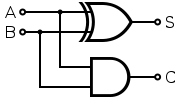
\includegraphics[scale=1]{\CURPATH/half_adder.png}
\caption{Half-adder}
\end{figure}

( The image has been taken from \href{https://en.wikipedia.org/wiki/Adder_(electronics)}{Wikipedia}. )

Full-adder:

% FIXME: TikZ!
\begin{figure}[H]
\centering
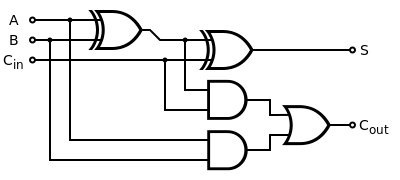
\includegraphics[scale=1]{\CURPATH/full_adder.png}
\caption{Full-adder}
\end{figure}

( The image has been taken from \href{https://en.wikipedia.org/wiki/Adder_(electronics)}{Wikipedia}. )

Here is a 4-bit ripple-carry adder:

% TikZ!
\begin{lstlisting}
         X3 Y3              X2 Y2              X1 Y1              X0 Y0
         |  |               |  |               |  |               |  |
         v  v               v  v               v  v               v  v
        +----+             +----+             +----+             +----+
Cout <- | FA | <- carry <- | FA | <- carry <- | FA | <- carry <- | HA |
        +----+             +----+             +----+             +----+
          ^                  ^                  ^                  ^
          |                  |                  |                  |
          S3                 S2                 S1                 S0
\end{lstlisting}

It can be used for most tasks.

Here is a 4-bit ripple-carry adder with carry-in:

\begin{lstlisting}
         X3 Y3              X2 Y2              X1 Y1              X0 Y0
         |  |               |  |               |  |               |  |
         v  v               v  v               v  v               v  v
        +----+             +----+             +----+             +----+
Cout <- | FA | <- carry <- | FA | <- carry <- | FA | <- carry <- | FA | <- Cin
        +----+             +----+             +----+             +----+
          ^                  ^                  ^                  ^
          |                  |                  |                  |
          S3                 S2                 S1                 S0
\end{lstlisting}

What carries are?
4-bit adder can sum up two numbers up to 0b1111 (15).
15+15=30 and this is 0b11110, i.e., 5 bits. Lowest 4 bits is a sum.
5th most significant bit is not a part of sum, but is a carry bit.

If you sum two numbers on x86 CPU, CF flag is a carry bit connected to \ac{ALU}.
It is set if a resulting sum is bigger than it can be fit into result.

Now you can also need carry-in.
Again, x86 CPU has ADC instruction, it takes CF flag state.
It can be said, CF flag is connected to adder's carry-in input.
Hence, combining two ADD and ADC instructions you can sum up 128 bits on 64-bit CPU.

By the way, this is a good explanation of "carry-ripple".
The very first full-adder's result is depending on the carry-out of the previous full-adder.
Hence, adders cannot work in parallel.
This is a problem of simplest possible adder, other adders can solve this.

To represent full-adders in CNF form, we can use Wolfram Mathematica.
I've taken truth table for full-adder from \href{https://en.wikipedia.org/wiki/Adder_(electronics)}{Wikipedia}:

% FIXME: table!
\begin{lstlisting}
Inputs 	|  Outputs
--------+----------
A B Cin |  Cout Sum
0 0 0   |  0    0
0 0 1   |  0    1
0 1 0   |  0    1
0 1 1   |  1    0
1 0 0   |  0    1
1 0 1   |  1    0
1 1 0   |  1    0
1 1 1   |  1    1
\end{lstlisting}

In Mathematica, I'm setting "->1" if row is correct and "->0" if not correct.

\begin{lstlisting}
In[59]:= FaTbl = {{0, 0, 0, 0, 0} -> 1, {0, 0, 0, 0, 1} -> 
   0, {0, 0, 0, 1, 0} -> 0, {0, 0, 0, 1, 1} -> 0, {0, 0, 1, 0, 0} -> 
   0, {0, 0, 1, 0, 1} -> 1, {0, 0, 1, 1, 0} -> 0, {0, 0, 1, 1, 1} -> 
   0, {0, 1, 0, 0, 0} -> 0, {0, 1, 0, 0, 1} -> 1, {0, 1, 0, 1, 0} -> 
   0, {0, 1, 0, 1, 1} -> 0, {0, 1, 1, 0, 0} -> 0, {0, 1, 1, 0, 1} -> 
   0, {0, 1, 1, 1, 0} -> 1, {0, 1, 1, 1, 1} -> 0, {1, 0, 0, 0, 0} -> 
   0, {1, 0, 0, 0, 1} -> 1, {1, 0, 0, 1, 0} -> 0, {1, 0, 0, 1, 1} -> 
   0, {1, 0, 1, 0, 0} -> 0, {1, 0, 1, 0, 1} -> 0, {1, 0, 1, 1, 0} -> 
   1, {1, 0, 1, 1, 1} -> 0, {1, 1, 0, 0, 0} -> 0, {1, 1, 0, 0, 1} -> 
   0, {1, 1, 0, 1, 0} -> 1, {1, 1, 0, 1, 1} -> 0, {1, 1, 1, 0, 0} -> 
   0, {1, 1, 1, 0, 1} -> 0, {1, 1, 1, 1, 0} -> 0, {1, 1, 1, 1, 1} -> 1}

...

In[60]:= BooleanConvert[
 BooleanFunction[FaTbl, {a, b, cin, cout, s}], "CNF"]

Out[60]= (! a || ! b || ! cin || s) && (! a || ! b || 
   cout) && (! a || ! cin || cout) && (! a || cout || s) && (a || b ||
    cin || ! s) && (a || b || ! cout) && (a || 
   cin || ! cout) && (a || ! cout || ! s) && (! b || ! cin || 
   cout) && (! b || cout || s) && (b || 
   cin || ! cout) && (b || ! cout || ! s) && (! cin || cout || 
   s) && (cin || ! cout || ! s)
\end{lstlisting}

These clauses can be used as full-adder.

Here is it:

\begin{lstlisting}
    # full-adder, as found by Mathematica using truth table:
    def FA (self, a,b,cin):
        s=self.create_var()
        cout=self.create_var()

        self.add_clause([self.neg(a), self.neg(b), self.neg(cin), s])
        self.add_clause([self.neg(a), self.neg(b), cout])
        self.add_clause([self.neg(a), self.neg(cin), cout])
        self.add_clause([self.neg(a), cout, s])
        self.add_clause([a, b, cin, self.neg(s)])
        self.add_clause([a, b, self.neg(cout)])
        self.add_clause([a, cin, self.neg(cout)])
        self.add_clause([a, self.neg(cout), self.neg(s)])
        self.add_clause([self.neg(b), self.neg(cin), cout])
        self.add_clause([self.neg(b), cout, s])
        self.add_clause([b, cin, self.neg(cout)])
        self.add_clause([b, self.neg(cout), self.neg(s)])
        self.add_clause([self.neg(cin), cout, s])
        self.add_clause([cin, self.neg(cout), self.neg(s)])

        return s, cout
\end{lstlisting}

And the adder:

\begin{lstlisting}
    # bit order: [MSB..LSB]
    # n-bit adder:
    def adder(self, X,Y):
        assert len(X)==len(Y)
        # first full-adder could be half-adder
        # start with lowest bits:
        inputs=my_utils.rvr(list(zip(X,Y)))
        carry=self.const_false
        sums=[]
        for pair in inputs:
            # "carry" variable is replaced at each iteration.
            # so it is used in the each FA() call from the previous FA() call.
            s, carry = self.FA(pair[0], pair[1], carry)
            sums.append(s)
        return my_utils.rvr(sums), carry
\end{lstlisting}

\subsubsection{Binary multiplier in SAT}

Remember school-level long division?
This multiplier works in a same way, but for binary digits.

Here is example of multiplying 0b1101 (X) by 0b0111 (Y):

% TikZ!
\begin{lstlisting}
         LSB
          |
          v
       1101 <- X
       -------
LSB 0|    0000
    1|   1101
    1|  1101
    1| 1101
    ^
    |
    Y
\end{lstlisting}

If bit from Y is zero, a row is zero.
If bit from Y is non-zero, a row is equal to X, but shifted each time.
Then you just sum up all rows (which are called "partial products".)

This is 4-bit binary multiplier. It takes 4-bit inputs and produces 8-bit output:

% FIXME: TikZ!
\begin{figure}[H]
\centering
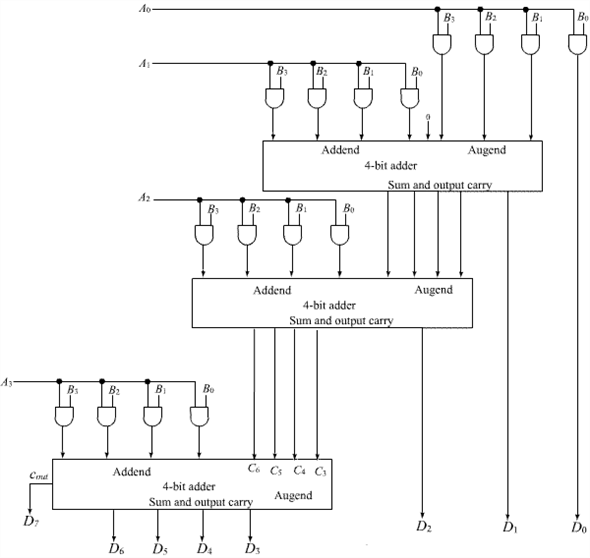
\includegraphics[scale=1]{\CURPATH/bin_mult.png}
\caption{4-bit binary multiplier}
\end{figure}

( The image has been taken from \url{http://www.chegg.com/homework-help/binary-multiplier-multiplies-two-unsigned-four-bit-numbers-u-chapter-4-problem-20p-solution-9780132774208-exc}. )

I would build separate block, "multiply by one bit" as a latch for each partial product:

\begin{lstlisting}
    def AND_Tseitin(self, v1, v2, out):
        self.add_clause([self.neg(v1), self.neg(v2), out])
        self.add_clause([v1, self.neg(out)])
        self.add_clause([v2, self.neg(out)])
    
    def AND(self,v1, v2):
        out=self.create_var()
        self.AND_Tseitin(v1, v2, out)
        return out

...

    # bit is 0 or 1.
    # i.e., if it's 0, output is 0 (all bits)
    # if it's 1, output=input
    def mult_by_bit(self, X, bit):
        return [self.AND(i, bit) for i in X]

    # bit order: [MSB..LSB]
    # build multiplier using adders and mult_by_bit blocks:
    def multiplier(self, X, Y):
        assert len(X)==len(Y)
        out=[]
        #initial:
        prev=[self.const_false]*len(X)
        # first adder can be skipped, but I left thing "as is" to make it simpler
        for Y_bit in my_utils.rvr(Y):
            s, carry = self.adder(self.mult_by_bit(X, Y_bit), prev)
            out.append(s[-1])
            prev=[carry] + s[:-1]
    
        return prev + my_utils.rvr(out)
\end{lstlisting}

AND gate is constructed here using Tseitin transformations.
This is quite popular way of encoding gates in CNF form, by adding additional variable:
\url{https://en.wikipedia.org/wiki/Tseytin_transformation}.
In fact, full-adder can be constructed without Mathematica, using logic gates, and encoded by Tseitin transformation.

\subsubsection{Glueing all together}

\lstinputlisting{\CURPATH/factor_SAT.py}
I just connect our number to output of multiplier and ask SAT solver to find inputs.
If it's UNSAT, this is prime number.
Then we factor factors recursively.

Also, we want block input factors of 1, because obviously, we do not interesting in the fact that n*1=n.
I'm using wide OR gates for this.

Output:

\begin{lstlisting}
 % python factor_SAT.py
factoring 1234567890
input_bits=31
factors of 1234567890 are 2 and 617283945
factoring 2
input_bits=1
2 is prime (unsat)
factoring 617283945
input_bits=30
factors of 617283945 are 3 and 205761315
factoring 3
input_bits=2
3 is prime (unsat)
factoring 205761315
input_bits=28
factors of 205761315 are 3 and 68587105
factoring 3
input_bits=2
3 is prime (unsat)
factoring 68587105
input_bits=27
factors of 68587105 are 5 and 13717421
factoring 5
input_bits=3
5 is prime (unsat)
factoring 13717421
input_bits=24
factors of 13717421 are 3607 and 3803
factoring 3607
input_bits=12
3607 is prime (unsat)
factoring 3803
input_bits=12
3803 is prime (unsat)
[2, 3, 3, 5, 3607, 3803]
\end{lstlisting}

So, $1234567890 = 2 \cdot 3 \cdot 3 \cdot 5 \cdot 3607 \cdot 3803$.

It works way faster than by Z3 solution, but still slow.
It can factor numbers up to maybe $\textasciitilde{}2^{40}$, while Wolfram Mathematica can factor
$\textasciitilde{}2^{80}$ easily.

% FIXME URL
The full source code: \url{.../factor_SAT.py}.

\subsubsection{Division using multiplier}

Hard to believe, but why we couldn't define one of factors and ask SAT solver to find another factor?
Then it will divide numbers!
But, unfortunately, this is somewhat impractical, since it will work only if remainder is zero:

\lstinputlisting{\CURPATH/div.py}

% FIXME URL
The full source code: \url{.../div.py}.

It works very fast, but still, slower than conventional ways.

\subsubsection{Breaking \ac{RSA}}

It's not a problem to build multiplier with 4096 bit inputs and 8192 output, but it will not work in practice.
Still, you can break toy-level demonstrational RSA problems with key less than $2^{40}$ or something like that
(or larger, using Wolfram Mathematica).

\subsubsection{Further reading}

% better titles
\href{https://yurichev.com/mirrors/SAT_factor/Encoding%20Basic%20Arithmetic%20Operations%20for%20SAT-Solvers.pdf}{1},
\href{https://yurichev.com/mirrors/SAT_factor/Factoring%20integers%20with%20parallel%20SAT%20solvers.pdf}{2},
\href{https://yurichev.com/mirrors/SAT_factor/Hard%20Instance%20Generation%20for%20SAT.pdf}{3}.

